\section{Cipher Specifications}

\begin{frame}{S-box}

\begin{itemize}
    \item Mysterion uses S-boxes that has bitslice representation with a combination of AND (also OR) and XOR gates. 
    \item It has a bitslice representation of 4 AND (precisely 3 AND and 1 OR) gates and 4 XOR gates
    \item It has a  differential probability of $2^{-2}$ and linear probability $2^{-1}$
\end{itemize}
\end{frame}

\begin{frame}{DDT \& LAT}
    \begin{figure}
    \centering
    \begin{subfigure}{}
      \centering
      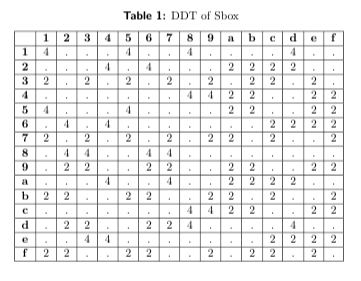
\includegraphics[scale=0.37]{DDT.png}
      \label{fig:sub1}
    \end{subfigure}%
    \begin{subfigure}{}
      \centering
      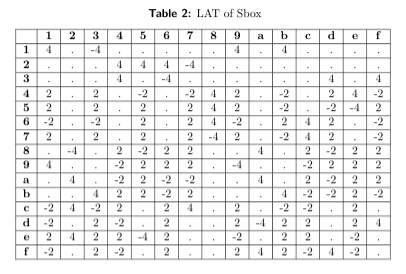
\includegraphics[scale=0.38]{LAT.png}
      \label{fig:sub2}
    \end{subfigure}
    \label{fig:test}
    \end{figure}
    \begin{block} {Observations}
    Differential probability = $\dfrac{4}{16}$ = $2^{-2}$ \\
    Linear probability = $\dfrac{4}{8}$ = $2^{-1}$ 
    \end{block}
\end{frame}

\begin{frame}{L-box}

    \begin{itemize}
        \item Its purpose is to diffuse changes in the state.
        \item linear transformation
        \item The algorithm which finds recursive MDS diffusion layers using shortened BCH codes from paper []
        \item When this is run using Magma code paper [] with $k =8$ and $s = 4$ as input gives polynomials whose companion matrix $C_m$ raised to power $8$ $\implies C^8_m$ gives us the MDS matrix 
     \end{itemize}
\end{frame}
\begin{frame}{Shift Columns}

    \begin{itemize}
        \item In Mysterion-128, as there are 4 blocks (with each block having 8 columns) ShiftColumns acts on columns two by two.
        \item In Mysterion-256 as there are 8 blocks (with each block having 8 columns) ShiftColumns acts on columns one by one
    \end{itemize}
\end{frame}

\begin{frame}{Diagrams}


\begin{center}
\begin{figure}[h!]
  \caption{Shift Columns-128}
   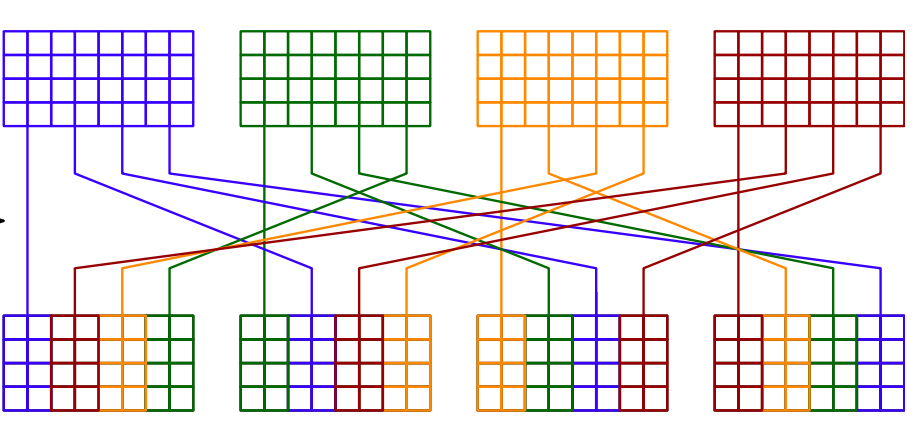
\includegraphics[width=6cm\textwidth]{128.png} 
\end{figure}
   
\end{center}

\begin{center}
\begin{figure}[h!]
  \caption{Shift Columns-256}
   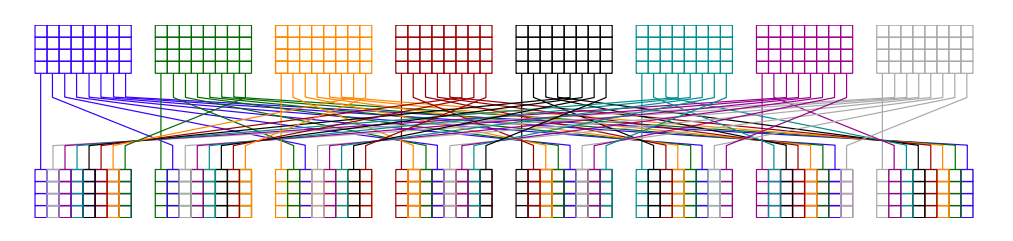
\includegraphics[width=10cm\textwidth]{256.png} 
\end{figure}
\end{center}

\end{frame}

\begin{frame}{Round constant and Key}
    \begin{itemize}
        \item Up until now, we have done nothing to make the ciphertext dependent on the key. So to do this, we add the key to the state. 
        \item The Mysterion block cipher has no key schedule. In every round, the same key is added to the state.
    \end{itemize}
\end{frame}